\section{Методы решения задачи}

В рамках проблемы извлечения аргументации необходимо решить две подзадачи: выделение структуры аргумента и определение полемической позиции. Обе эти задачи являются задачами классификации. Формально даны два текста (предложения) $A = (a_1, a_2, ..., a_n)$ и $B = (b_1, b_2, ..., b_m)$, где $a_i, b_j$ - слова. Необходимо для пары компонент аргументации $A,B$ определить класс отношения $Y = (y_1, ..., y_k)$, т.е. смоделировать функцию ($P$ обозначает вероятность):

\begin{equation*}
    f(A, B, y_i) = P(y_i| A, B)
\end{equation*}

В задаче определения структуры аргументации присутствует два класса: отношение релевантности и нерелевантности (нейтральное). В задаче определения полемической позиции также два одношения: поддержка и опровержение (атака).

В задаче определения пропаганды присутствует 14 классов пропаганды, постановка задачи остается похожей: дан новостной текст $X = (x1, ..., x_n)$, дан участок $x_i, ..., x_i + k$, необходимо классифицировать данный сегмент в один из классов $Y = (y_1, ..., y_14)$:
\begin{itemize}
    \item Сильно окрашенная лексика. Пример: ".. a lone lawmaker’s childish shouting."
    \item Навешивание ярлыков и имен. Пример: "Republican congressweasels"
    \item Повторение. Заключается в повторении тезиса для закреплении концепции в голове у слушателей.
    \item Преувеличение или приуменьшение. Пример: "Democrats bolted as soon as Trump’s speech ended in an apparent effort to signal they can’t even stomach being in the same room as the president"
    \item Сомнения. Пример: "Is he ready to be the Mayor?"
    \item Взывание к страхам и предрассудкам. Пример: "stop those refugees; they are terrorists"
    \item Сбор под флагом, т.е. взывание к аудитории на почве общей какой-либо общей идентичности (национальности, пола и т.п.). Пример: "entering this war will make us have a better future in our country"
    \item Упрощение причины, т.е. упор на какую-либо первопричину в проблеме с множеством факторов. Пример: "If France had not declared war on Germany, World War II would have never happened."
    \item Слоганы - любые яркие фразы, взывающие к эмоциям. Пример: "Make America great again!"
    \item Диктатура - представление ограниченного выбора в задаче, где существует большее число вариантов решение проблемы. Пример: "There is no alternative to war."
    \item Терминирующие размышления клише - фразы дискредитирующие критичекское размышление по теме обсуждения. Пример: "никто не идеален" или "нельзя изменить человеческую натуру"
    \item Whataboutism - перевод темы для занятия более высокой моральной позиции. Пример: "А у вас права ущемляют!".
    \item Сведение вопроса к заведомо осуждаемой теме. Пример: "Only one kind of person can think this way: a communist!"
    \item Красная сельдь - представление нерелевантной информации для отвращения внимания. 
    \item Стадность - захват мнения через представление позиции, как поддерживаемой большинством. Пример: "Would you vote for Clinton as president? 57\% say yes."
    \item Нарочитая расплывчатость и неясность.
    \item Соломенный человек - подстановка похожего утверждения вместо утверждения оппонента с его последующим опровержением.
\end{itemize}

В задаче извлечения пропаганды дополнительно стоит задача нахождения участков текста, являющихся пропагандой, т.е. для текста $X = (x_1, ..., x_n)$ определить бинарный набор меток $Y = (y_1, ..., y_n)$, где $y_i = 1$, если слово $x_i$ входит в сегмент с пропагандой, иначе $y_i = 0$. Для решения проблемы необходимо построить модель:

\begin{equation*}
    f(X, Y) = P((y_1, y_2, ..., y_n) | (x_1, x_2, ..., x_n))
\end{equation*}

\subsection{Современные подходы к обработке естественного языка}
За последнее десятилетие область обработки текстов значительным образом преобразилась. Тексты хуже поддаются обработке различными нейросетевыми алгоритмами из-за их дискретной структуры. Ранние работы, основаные на классических метотдах машинного обучения используют методики Bag of words или Tf-Idf для векторизации текста. Данные подходы не способны улавливать сложные закономерности, так как не учитывают порядок и внутреннюю структуру текста, поэтому их зачастую дополняют информацией о синтаксической структуре предложения и другуми экспертными признаками.

В 2013 году с появлением word2vec \cite{mikolov2013efficient} началось стремительное развитие применения нейросетей в обработке текстов. Основная идея данного подхода заключается в выучивании векторов слов для моделирования дистрибутивной гипотезы: слова, встречающиеся в схожих контекстах, имеют близкие значения.

Долгое время стандартом моделей была одна из векторизаций (word2vec, glove, fasttext) дополненная рекуррентной нейросетью (LSTM, GRU) \cite{hochreiter1997lstm} и финальным слоем специфичным для задачи.  В данном подходе рекуррентные нейросети выучивыают контекстные закономерности в рамках определенной задачи.

Со временем начали появляться модели общего назначения для задачи восприятия естественного языка (Natural Language Understanding). Данные модели не требуется обучать с нуля, вместо этого они проходят длительное предобучения на общей задаче моделирования языка \cite{Peters:2018}: для последовательности $X = (x_1, x_2, .., x_k)$ слов из словаря $V = (v_1, v_2, ..., v_n)$ моделируется следующая закономерность:

\begin{equation*}
    f(X, v_i) = P(x_{k+1} = v_i| (x_1, ..., x_k))
\end{equation*}

В настоящий момент большие предобученные модели основанные на архитектуре трансформер являются доминирующими почти во всех областях обработки текстов. Особенностью данной архитектуры является полный отказ от рекуррентности в пользу механизма внимания.

Механизм внимания пришел из задачи машинного перевода, где главным подходом была архитектура Seq2Seq \cite{sutskever2014sequence}. Данная архитектура состоит из энкодера, сжимающего предложение в вектор, и декодера, разжимающего данный вектор в текст на другом языке. Одна из главных заявленнных проблем - данный подход плохо работает на длинных предложениях. Это связано с тем, что при сжатии в вектор фиксированного размера теряется очень большой объем информации.

Прорыв произошел с разработкой механизма внимания \cite{bahdanau2014neural}. Данный механизм позволяет сопоставлять вектор предложения в декодере с соответствующими состояними в энкодере. Каждому состоянию энкодера, соответствуещему определенному токену, на каждом шаге при декодировке ставится в соответствие вес, после чего состояния энкодера усредняются с данными весами и используются для расширения внутреннего состояния декодера.

Архитектура трансформер \cite{vaswani2017attention} основывается на механизме внимания. В рамках нейросетевой модели механизм внимания применяется от каждого слова предложения ко всем словам предложения. С последовательным применением нелинейности данный механизм применяется несколько раз на каждом слое нейросети, после чего на выходе получается векторное представление для каждого слова в предложении, насыщенное контекстуальной информацией.

Одной из самых популярных предобученных архитектур является BERT \cite{devlin2018bert}. Данная модель обучалась на коллекции Book Corpus задаче маскированного языкового моделирования и предсказания следующего предложения. Задача маскированного языкового  моделирования заключается в предсказании одного и более слов в предложении. Таким образом после обучения модель имеет внутри себя знания о структуре языка, о мире, поэтому ее легко адаптировать для различных вариаций задачи понимания естественного языка.

Это подтверждается успехом подобных моделей почти во всех современных задачах естественного языка и особом соревновании GLUE Benchmark. Данное соревнование содержит в себе ряд задач на понимание языка, которые при небольшом дообучении решаются моделями подобными BERT на уровне человека или выше.

В рамках данной работы было выбрано использовать нейросетевые подходы на основе предобученных моделей-трансформеров, так как данные модели показывают наилучшие результаты на большинтстве задач обработки естественного языка.

\subsection{Модели для извлечения аргументации}
Для извлечения аргументации необходимо решить подзадачи построения структуры и определения полемической позиции аргументации. В рамках рассмотренных корпусов компонентами аргументации являются темы и утверждения или предпосылки. Стоит дополнительно отметить, что не у всех представленных текстовых коллекций присутствуют какие-либо базовые решения и замеры качеств.

В работе, сопровождающей корпус IBM Claim Stance \cite{bar2017stance} предложенная модель представляет собой метод опорных векторов (Support Vector Machine) над векторизацией мешка слов (Bag of words). 

В работе \cite{toledo2020multilingual} для определения полемической позиции, структуры и качества аргумента предлагается система, основанная на предобученной модели $BERT$, однако сама архитектура не раскрывается.

Отсутствие предложенных базовых решений приводит к необходимости использования заимствованных или альтернативных подходов. Для классификации отношений между двумя парами компонент аргументации предлагается модель $BERT_{basic}$. В рамках данной модели входы, представляющие из себя две компоненты аргументации объединяются в один текст, разделенные специальным символом \textbf{[SEP]}. После этого входная последовательность проходит сквозь слои модели, в результате чего механизм внимания, интерпретируя закономерности между двумя текстами, выдает сжатый вектор. Далее данный вектор подается в линейный слой, который решает задачу классификации.

Данная модель вдохновлена оригинальной методикой предобучения модели $BERT$, в которой аналогичным образом решалась задача предсказания следующего предложения (Next sentence prediction) - необходимо было определить, является ли одно предложение продолжением другого. 

Стоит отметить, что сложность работы модели квадратична относительно длины входной последовательности, и, возможно, данный подход не был бы эффективен в сценарии, где необходимо было бы быстро извлечь аргументацию из большого количества текстов. Альтернативой первой модели служит модель $BERT_{vectorized}$, в которой предлагается независимо пропустить две компоненты аргументации через слои предобученной модели, после чего сконкатенировать их векторные представления и передать для классификации в линейный слой. За счет уменьшения длины входных данных уменьшается и время работы модели, однако компоненты аргументации векторизуются без информации друг о друге, что может привести к потере качества.

В работе \cite{sun2020self} предлагается подход улучшения качества модели за счет добавления интерпретируемости. Данная модель $BERT_{SE}$ представляет собой дополненую модель $BERT_{basic}$: в конце после прохождения всех слоев трансформера для каждого слова на выходе имеется вектор, отображающий контекстуальную информацию предложения внутри текста, т.е. каждая входная последовательность $X = (x_1, ..., x_n)$ отображается в последовательность векторов $H = (h_1, ..., h_n), h_i = (h_{i_1}, ..., h_{i_k}$, где $k$ - размерность модели.
В обычной задаче классификации берется выход на первом слове $h_1$, т.е. на спецсимволе начала предложения \textbf{[CLS]}. В модели $BERT_{SE}$ предлагается взять всевозможные участки текста вида $span(i, j), i \leq j, |span(i, j)| = k$ и с помощью линейного слоя проставить каждому участку текста некое число $s_q$, отражающее важность данного участка текста в финальной классификации. После этого $s_q$ превращается в множители для взвешенной суммы участков текста, финальное векторное представление $t$ для классификации считается следующим образом:

\begin{equation*}
    \alpha_i = \frac{\exp(s_i)}{\sum_{j=1}^{k}\exp(s_j)} \\
\end{equation*}
\begin{equation*}
        t=\sum_{q=1, i \leq j}^{k} \alpha_q * span(i, j)
\end{equation*}
Далее взвешенное представление всех участков $t$ подается в линейный слой для решения задачи классификации. Множители $\alpha_i$ могут использоваться для интерпретации модели, так как они отображают самый важный для классификации непрерывный участок текста.


Дополнительн для исследования применимости знаний, полученных на корпусе SNLI предлагается обучить модель $BERT_{basic}$ на задаче логического вывода и исследовать следующие сценарии: применимость модели без дообучения на корпусах извлечения аргументации (Zero Shot) и исследование предобучения модели на корпусе SNLI для дообучения целевой задаче извлечения аргументации. 

\subsection{Модели для обнаружения пропаганды}
Задача извлечения пропаганды является новой задачей, к которой не было применено никаких существующих подходов. В дорожке по детекции, где было необходимо выделить участки текста, являющиеся пропагадной, было предложено начать с базовых моделей из работы \cite{lample2016neural}. Первая модель $LSTM$ основывается на одноименной архитектуре рекуррентных нейросетей. На вход модели подается текст, представляемый последовательностью слов $X = (x_1, .., x_n)$, после чего данный текст проходит через LSTM-слои и преобразуется в контекстные вектора $H = (h_1, ..., h_n), h_i = (h_{i_1}, ..., h_{i_k}$. Каждому слову на основе полученных векторов независимо ставится метка 0 (отсутствие пропаганды) или 1 (пропаганда) с помощью применения линейного слоя. Данные метки составляют список меток $Y = (y_1, ..., y_n)$, который однозначно определяет все участки пропаганды в тексте.

Модификацией данной модели является $LSTM_{CRF}$. Предлагается устранить недостатки предудыщей модели за счет замены финального слоя на слой Conditional Random Field (CRF). Данный слой выучивает возможные переходы и моделирует всю последовательнсть $Y$ одновременно.

В качестве более сложных моделей предлагается использовать предобученную модель $BERT$ для векторизации входной последовательности и аналогично с предыдущими моделями в качестве выходных слоев испытать и линейный слой и CRF.

Также было решено позаимствовать архитектуру $LaserTagger$ из работы \cite{malmi2019encode}, так как данная модель зарекомендовала себя для классификации длинных последовательностей. Основная идея модели заключается в том, чтобы аналогично задаче машинного перевода, используя архитектуру "encoder-decoder" поставить каждому слову соответствующую метку.

Для улучшения работы модели $LaserTagger$ было предложено два дополнительных механизма Label Smoothing и Teacher Forcing. Техника label smoothing заключается в преобразовании меток класса из 0 и в более "мягкие", такие как 0.2 и 0.8. Данная методика позволяет сгладить резкие изменения градиентов на ошибках модели. Teacher forcing заключается в подаче авторегрессионной модели не только правильрных меток, но и предсказанных ею неверных меток. Таким образом модель становится более устойчивой к ошибкам и исследуюет во время обучение больше различных сценариев. 

\begin{figure}[h!]
\centering
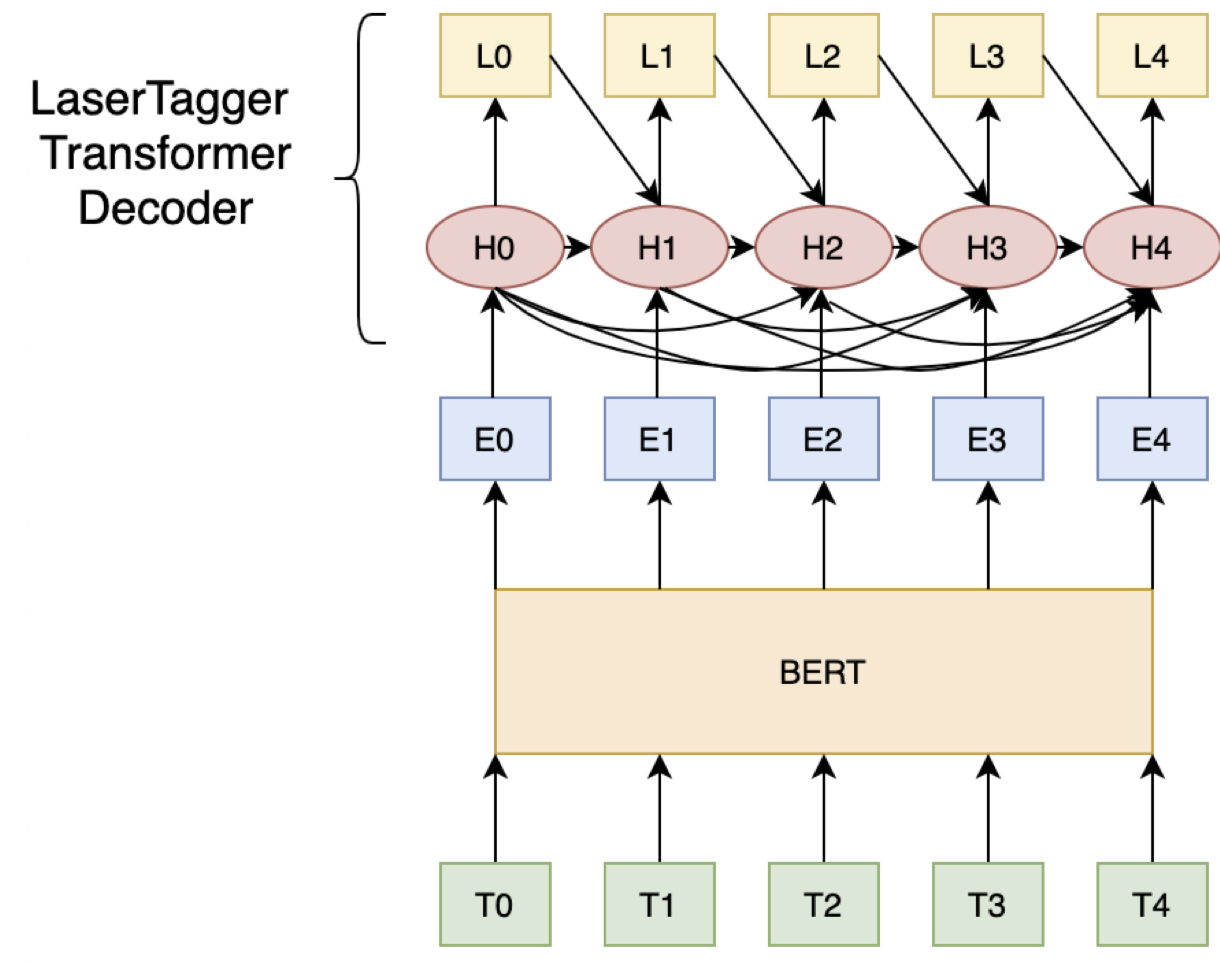
\includegraphics[scale=.5]{lasertagger.png}
\caption{Архитектура LaserTagger.}
\label{Problem_Picture}
\end{figure}


Во второй дорожке требовалось для каждого сегмента пропаганды определить, к каким классам он относится. Задача поставлена на уровне предложений, однако решать ее как классификацию предложений невозможно: в одном предложении может содержаться более одного участка пропаганды. Для этого было решено адаптировать модельный подход $RBERT$ \cite{wu2019enriching}, заключающийся в обрамлении нужных участков текста спецсимволами. Таким образом модели выделяется нужная фраза, что позволяет при необходимости работать с разными участками текста в рамках одного предложения.

\begin{figure}[h!]
\centering
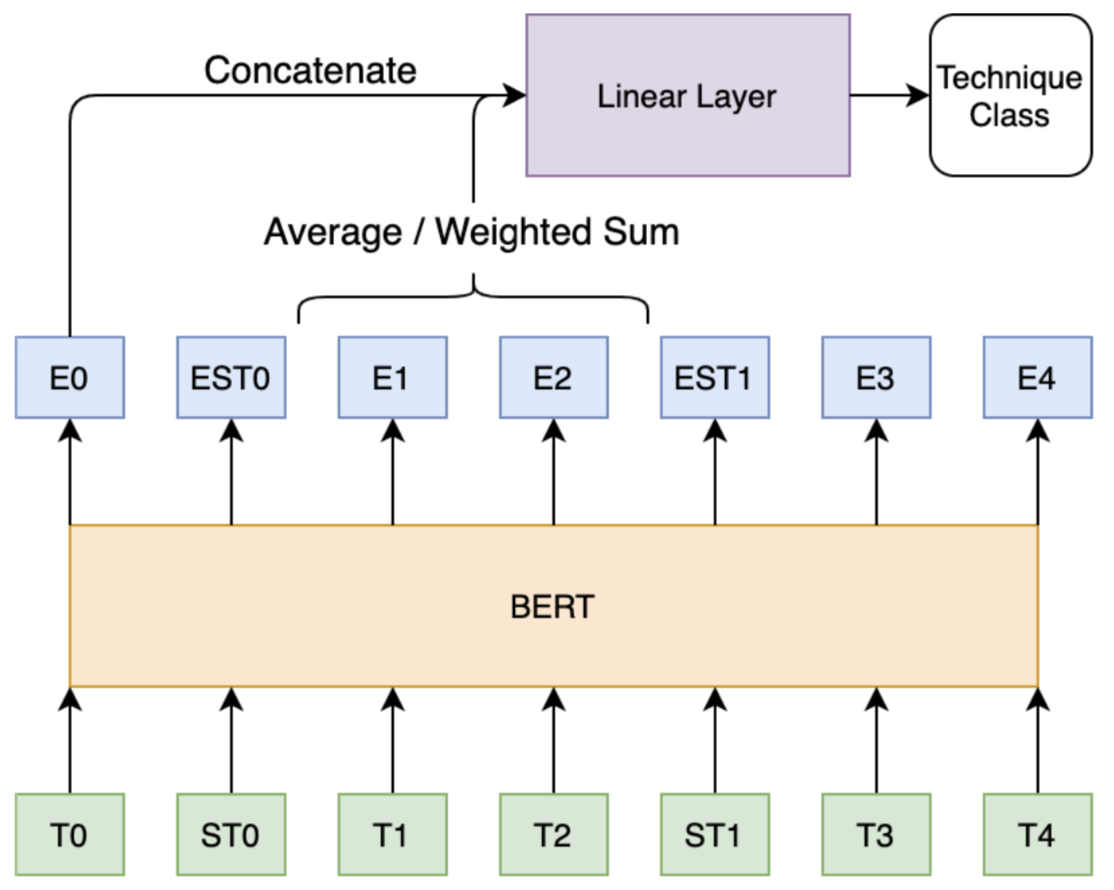
\includegraphics[scale=.5]{rbert.png}
\caption{архитектура R-BERT.}
\label{Problem_Picture}
\end{figure}


\subsection{Методы для межязыкового переноса знаний}

В области обработки естественного языка наиболее распространены англоязычные корпуса. Английский язык получает наибольшее покрытие задачами, однако проверка работоспособности моделей на других языках из-за этого остается плохо исследованной проблемой.

Методов получить модель для другого языка несколько, направления межязыкового переноса активно развивается в настоящее время. Самым простоым способом является создание параллельного корпуса. Использование профессиональных переводчиков затратно и треюует много времени, поэтому достаточно часто для первичной проверки гипотез прибегают к автоматизированным средствам перевода.

Второй подход заключается в адаптации мультиязычной модели, т.е. модели предобученной на корпусе из различных языков. Считается, что для представлений одних и тех же слов на разных языках модель имеет схожие векторные представления, которые "замораживаются", т.е. не обучаются дальше. После этого данная модель дообучается на конкретной задаче на тех языках, на которых данная задача доступна, а качество замеряется уже на целевом языке.


\subsection{Выводы}

В результате обзора современных нейросетевых подходов были выбраные следующие модели для задачи извлечения аргументации:
\begin{itemize}
    \item Модель $BERT_{basic}$, т.к. она является базовой вариацией модели классификации, основанной на больших предобученных моделях.
    \item Модель $BERT_{vectorized}$ для исследования важности применения механизма внимания между компонентами аргументации.
    \item Модель $BERT_{SE}$ для исследования интерпретируемости результатов.
\end{itemize}

Для извлечения пропаганды были предложены две модели:
\begin{itemize}
    \item Модель, основанная на рекуррентной нейросети $LSTM$, так как это хорошее базовое решение, зарекомендовавшее себя в задачах классификации последовательностей.
    \item Модель $LaserTagger$, так как она зарекомендовала себя на задачах классификации длинных последовательностей.
    \item Модель $RBERT$ для классификации участков текста, так как она позволяет выделить интересующий участок пропаганды.
\end{itemize}

Для исследования переноса знаний на русский язык было выбрано перевести корпус IBM Claim Stance с помощью автоматизированного сервиса Google Translate и применить подход с заморозкой входных слоев мультиязычной модели $BERT_{multilingual}$ для дальнейшего замера качества на переведенном корпусе.